\chapter{Referencial Teórico}

Este capítulo apresenta o referencial teórico estudado para que fosse possível realizar o desenvolvimento do simulador acústico proposto neste trabalho. São abordados neste capítulo, conceitos referentes a acústica, simulação, simulação acústica e sistemas multiagentes.

\section{Acústica}

Nesta seção serão apresentados alguns conceitos importantes sobre acústica que serão abordados neste projeto.

\subsection{Conceito do som}

Ao falarmos sobre som, existem dois conceitos importantes a serem tratados, o som vibração, ou pertubação física, que percorre um meio qualquer de propagação e o som, sensação sonora, psico-fisiológico, que é captado pelo nosso ouvido. O conceito que mais interessa aos profissionais da Acústica Arquitetônica é o último, isto é, o do som, sensação sonora, captada pelo nosso aparelho auditivo. \cite{silva}.

Segundo \citeonline[pág.~6]{bistafa}, o som pode ser definido como uma variação da pressão ambiente detectável pelo sistema auditivo.

Para que haja a propagação do som, é necessário que ele esteja em um meio de propagação, provido de inércia e de elasticidade. O meio mais comum desta propagação, para chegar até ao nosso ouvido, é o ar que nos envolve. Se não houver gás preenchendo o espaço que nos circunda, os sons deixarão de ser ouvidos. \cite{silva}

\subsection{Frequência}

Segundo \citeonline[pág.~34]{silva}, chama-se de frequência o número de oscilações completas por segundo, ou seja, o número de idas e voltas completas da partícula vibrante. A Frequência é medida em ciclos por segundo (c.p.s) ou em Hertz (Hz).

Se representarmos o diagrama das pressões para um ponto qualquer de um recinto, onde se propague o som, em função do tempo, encontraremos o gráfico da figura~\ref{grafico_frequencia}, onde as pressões foram registradas em ordenadas e o tempo em abcissas. As suas unidades são, respectivamente, $ dina/cm^{2} $ e $ segundo $. \cite{silva}

\begin{figure}[!htb]
\centering
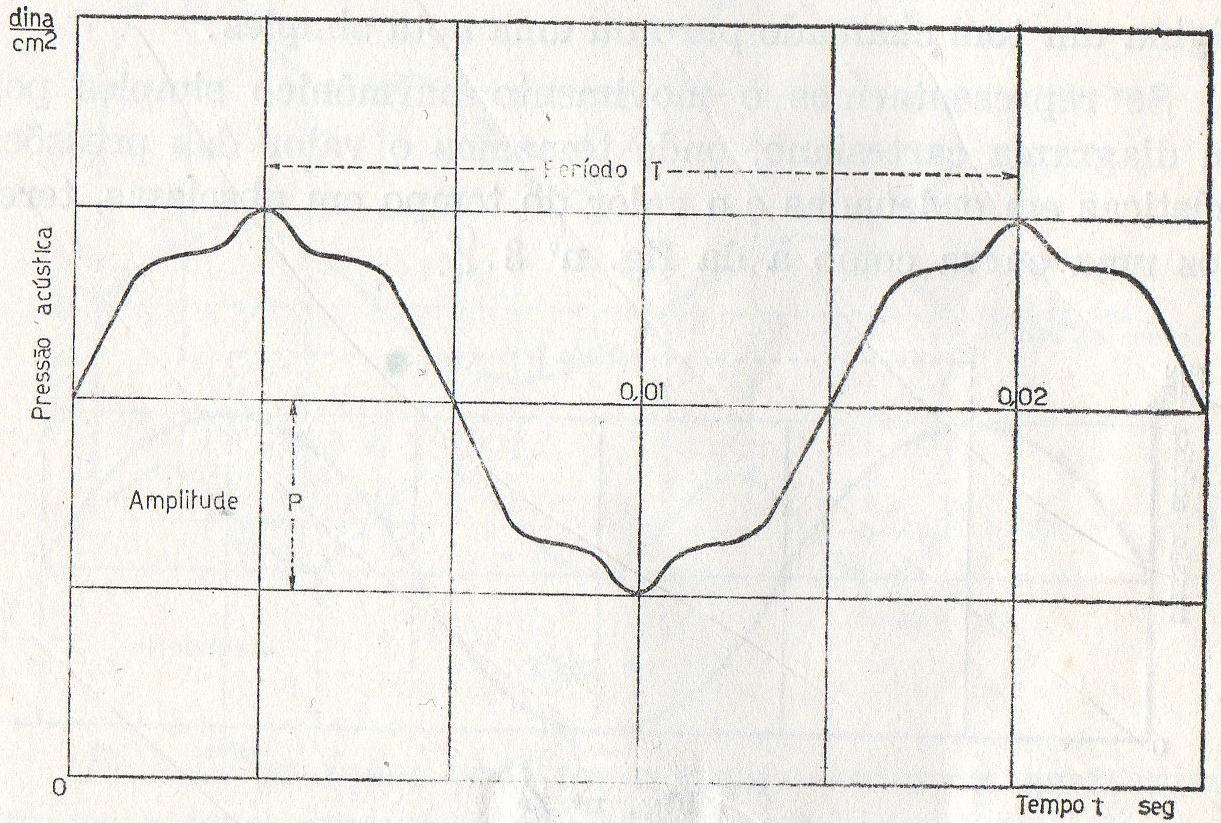
\includegraphics[scale=0.4]{figuras/grafico_frequencia}
\caption{Gráfico de frequência \cite{silva}}
\label{grafico_frequencia}
\end{figure}

O período T é o tempo necessário para se realizar uma oscilação completa. Portanto, sendo a frequência o número de períodos por segundo, a fórmula que exprime seu valor será \cite[pág.~7]{bistafa}:
\begin{center}
\begin{LARGE}
$ f = \frac{1}{T} $
\end{LARGE}
\end{center}

\begin{citacao}
\begin{normalsize}
"Os sons audíveis encontram-se no intervalo de $ \pm $ 16 a $ \pm $ 20.00 c.p.s. Aqueles, abaixo de 16 c.p.s, são chamados de infra-sons e aqueles, acima de 20.000 c.p.s, são designados como ultra-sons. Tanto uns como os outros não são captados pelo ouvido humano. \cite[pág.~35]{silva}." 
\end{normalsize}
\end{citacao}

Em música, o termo utilizado para a percepção da frequência sonora pelo ouvido humano é a altura. Quanto maior o número de oscilações por segundo, maior é a sua altura, portanto, as frequências baixas são percebidas como sons graves e as frequências mais altas como sons agudos.

\subsection{Intensidade sonora}

Para que possamos ter a sensação de audição, além da necessidade de o som estar entre o intervalo de 16 a 20.000 oscilações por segundo, isto é, ter determinada altura, é necessário que ele tenha uma certa intensidade sonora. \cite[pág~42]{silva}

Segundo \citeonline[pág~42]{silva}, a intensidade sonora $ I $, medida em $ watt/cm^{2} $, é a quantidade de energia sonora $ W $, medida em $ watt $, que atravessa um centímetro quadrado de área, perpendicular à direção em que o som se propaga. É calculada através da fórmula:

\begin{center}
\begin{Large}
$ I = \frac{W}{S} $
\end{Large}
\end{center}

A menor variação de pressão ambiente detectável pelo sistema auditivo é da ordem de $ 10^{-12}W/m^{2} $, também conhecido como limiar de audibilidade. Já a variação de pressão ambiente capaz de provocar dor é o limiar de dor, que é equivalente à $ 1W/m^{2} $. \cite[pág~6]{bistafa}

\begin{center}
\begin{Large}
$ I_{0} = 10^{-12}~W/m^{2} $
\end{Large}
\end{center}

\begin{center}
\begin{Large}
$ I_{máx} = 1~W/m^{2} $
\end{Large}
\end{center}

% (Falar sobre nível de intensidade sonora)...
Relacionado a intensidade sonora, existe também o conceito de nível de intensidade sonora, o qual é representado pelo decibél (dB) e é equivalente a uma relação percentual. O nível de intensidade sonora precisa de um valor de referência para ser expresso. Em acústica, o 0 dB é equivalente ao limiar de audibilidade e, a cada 10 dB, a intensidade sonora aumenta em dez vezes e dobra a cada aproximadamente 3 db. A expressão utilizada para calcular o nível de intensidade sonora com base na intensidade sonora é: 

\begin{center}
\begin{Large}
$ \beta = 10\log{\frac{I}{I_{0}}} $
\end{Large}
\end{center}

\subsection{Reflexão}

Quando uma onda sonora atinge uma parede ou um obstáculo qualquer, parte da energia incidente é refletida, parte é dissipada pelo obstáculo, transformando-se em energia calorífica ou mecânica. O restante atravessa o referido obstáculo, passando para o outro lado, transmitindo-se através do meio adjacente. \cite{silva}.

\begin{figure}[!htb]
\centering
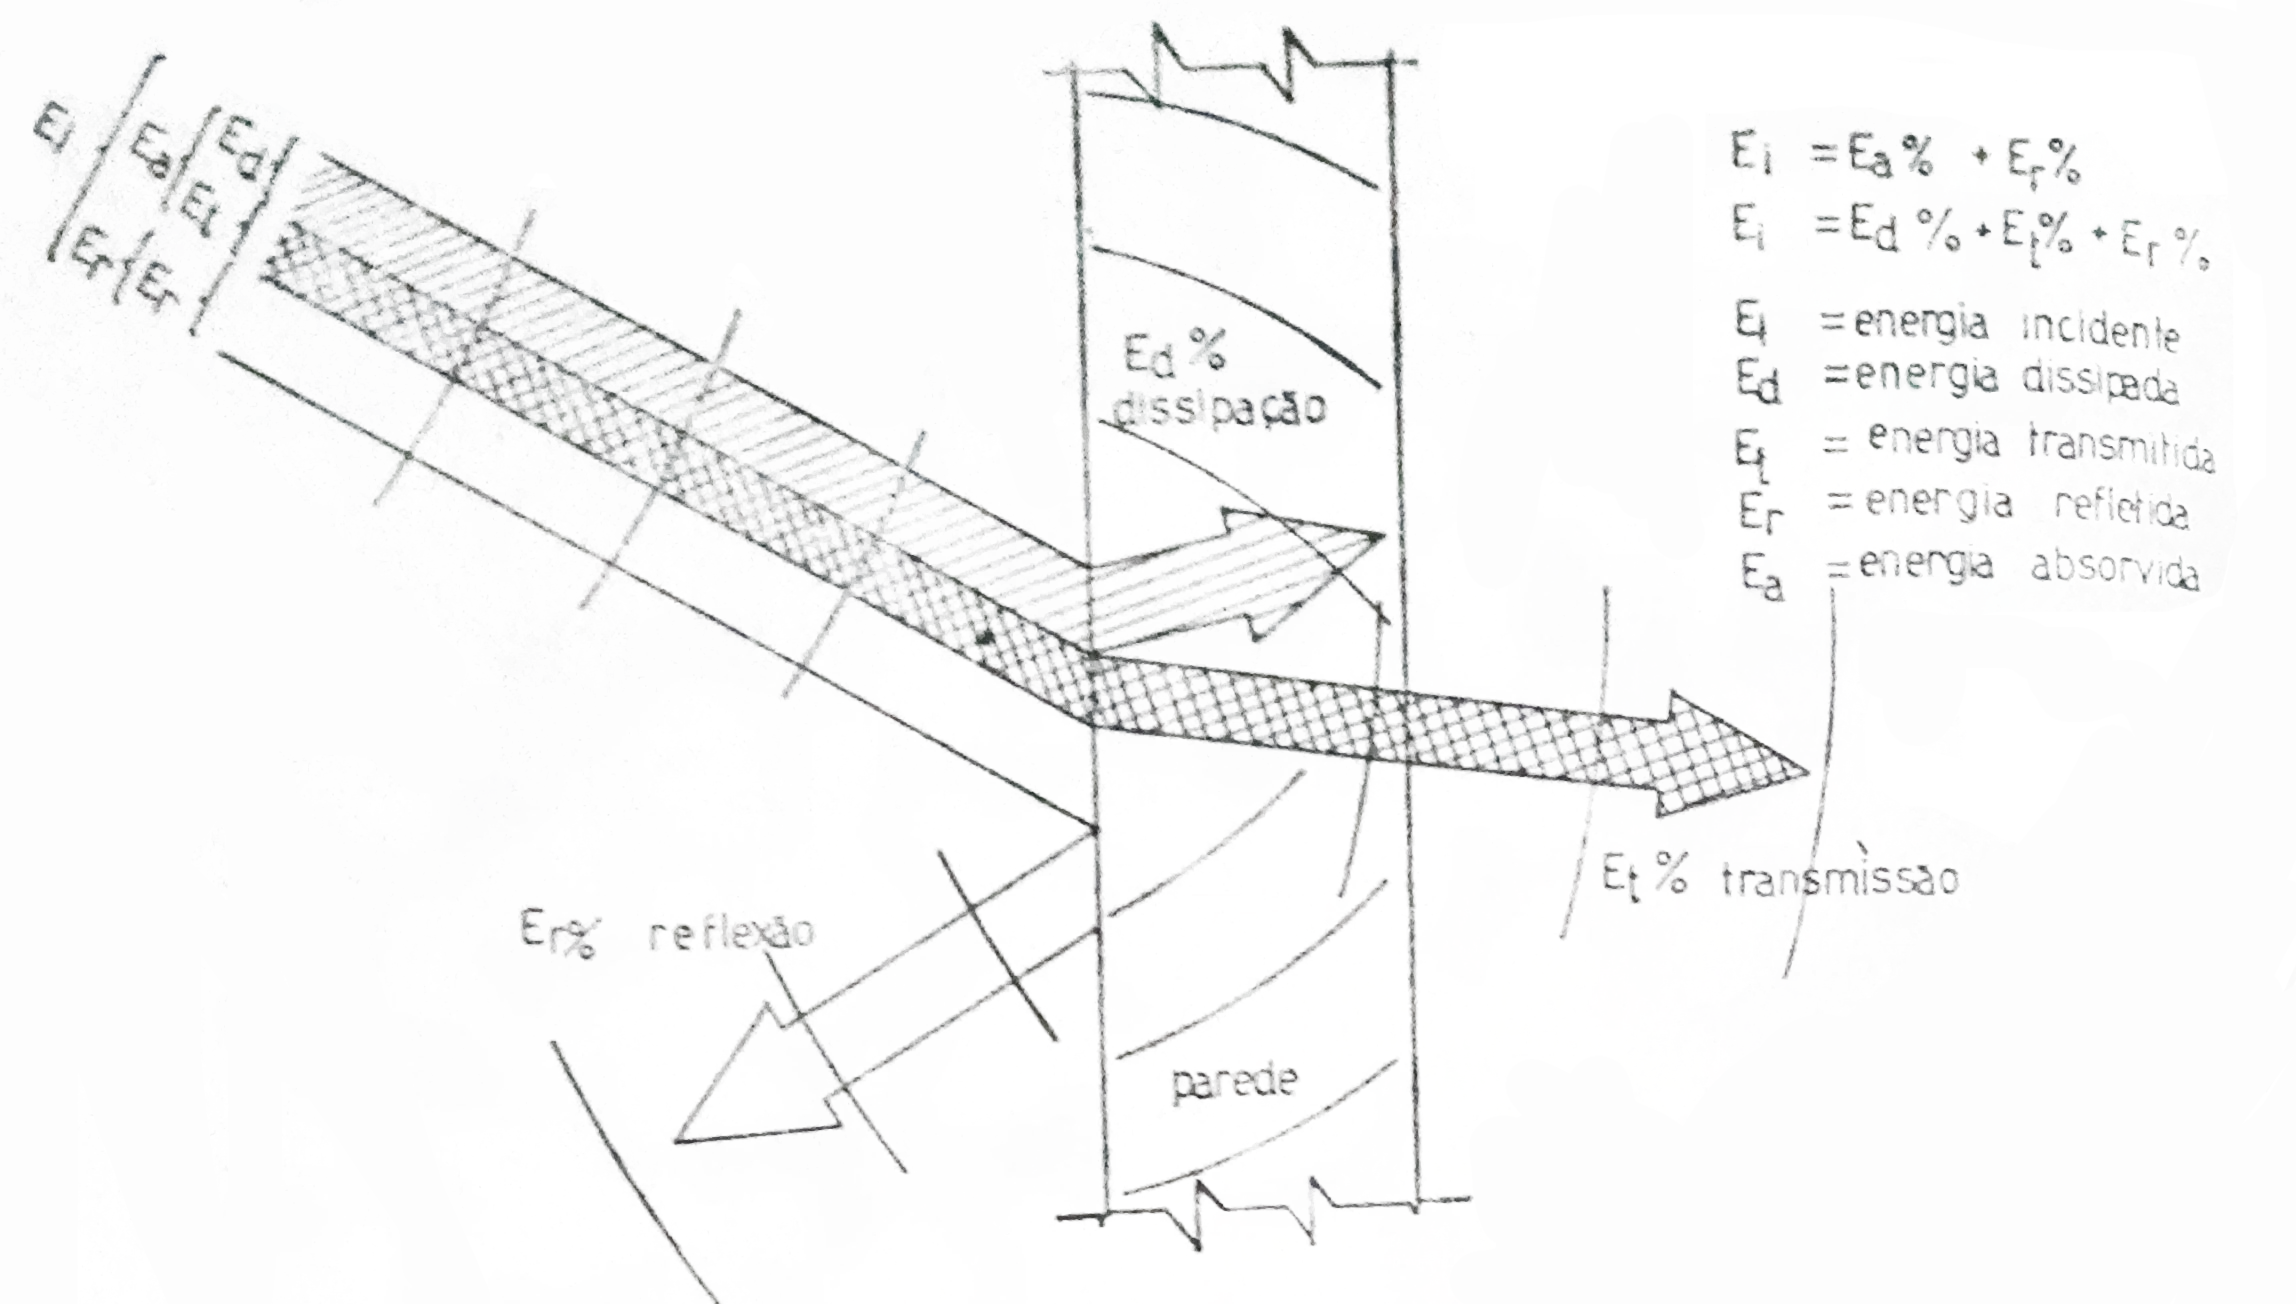
\includegraphics[scale=0.2]{figuras/Reflexao}
\caption{Transmissão, absorção e reflexão do som \cite{silva}}
\label{fig:reflexao}
\end{figure}

As paredes e divisões, geralmente rígidas, vibram no todo ou em parte, devido à energia das ondas sonoras. Essas paredes e divisões vibram como se fossem diafragmas e rerradiam a energia, que nelas incida. Sendo assim, as paredes ou divisões mais rígidas e mais pesadas são melhores isolantes sonoros, do que aquelas construídas de material leve e flexível. \cite[pág.~83]{silva}.

Segundo \citeonline[pág.~84]{silva}, quando uma onda sonora pura ou livre, isto é, isenta de reflexões secundárias, atinge uma superfície uniforme e relativamente grande, em relação ao comprimento dessa onda, a reflexão do som assemelha-se muito com à da luz.

Se representarmos as ondas sonoras pelos seus raios sonoros, elas serão retas dirigidas segundo a direção em que as mesmas caminham. \cite[pág.~84]{silva}

O ângulo do raio incidente, com a normal à superfície refletora, é igual ao ângulo formado pelo raio refletido com aquela mesma linha e estão no mesmo plano, conforme representado na figura \ref{fig:reflexao2}.

\begin{figure}[!htb]
\centering
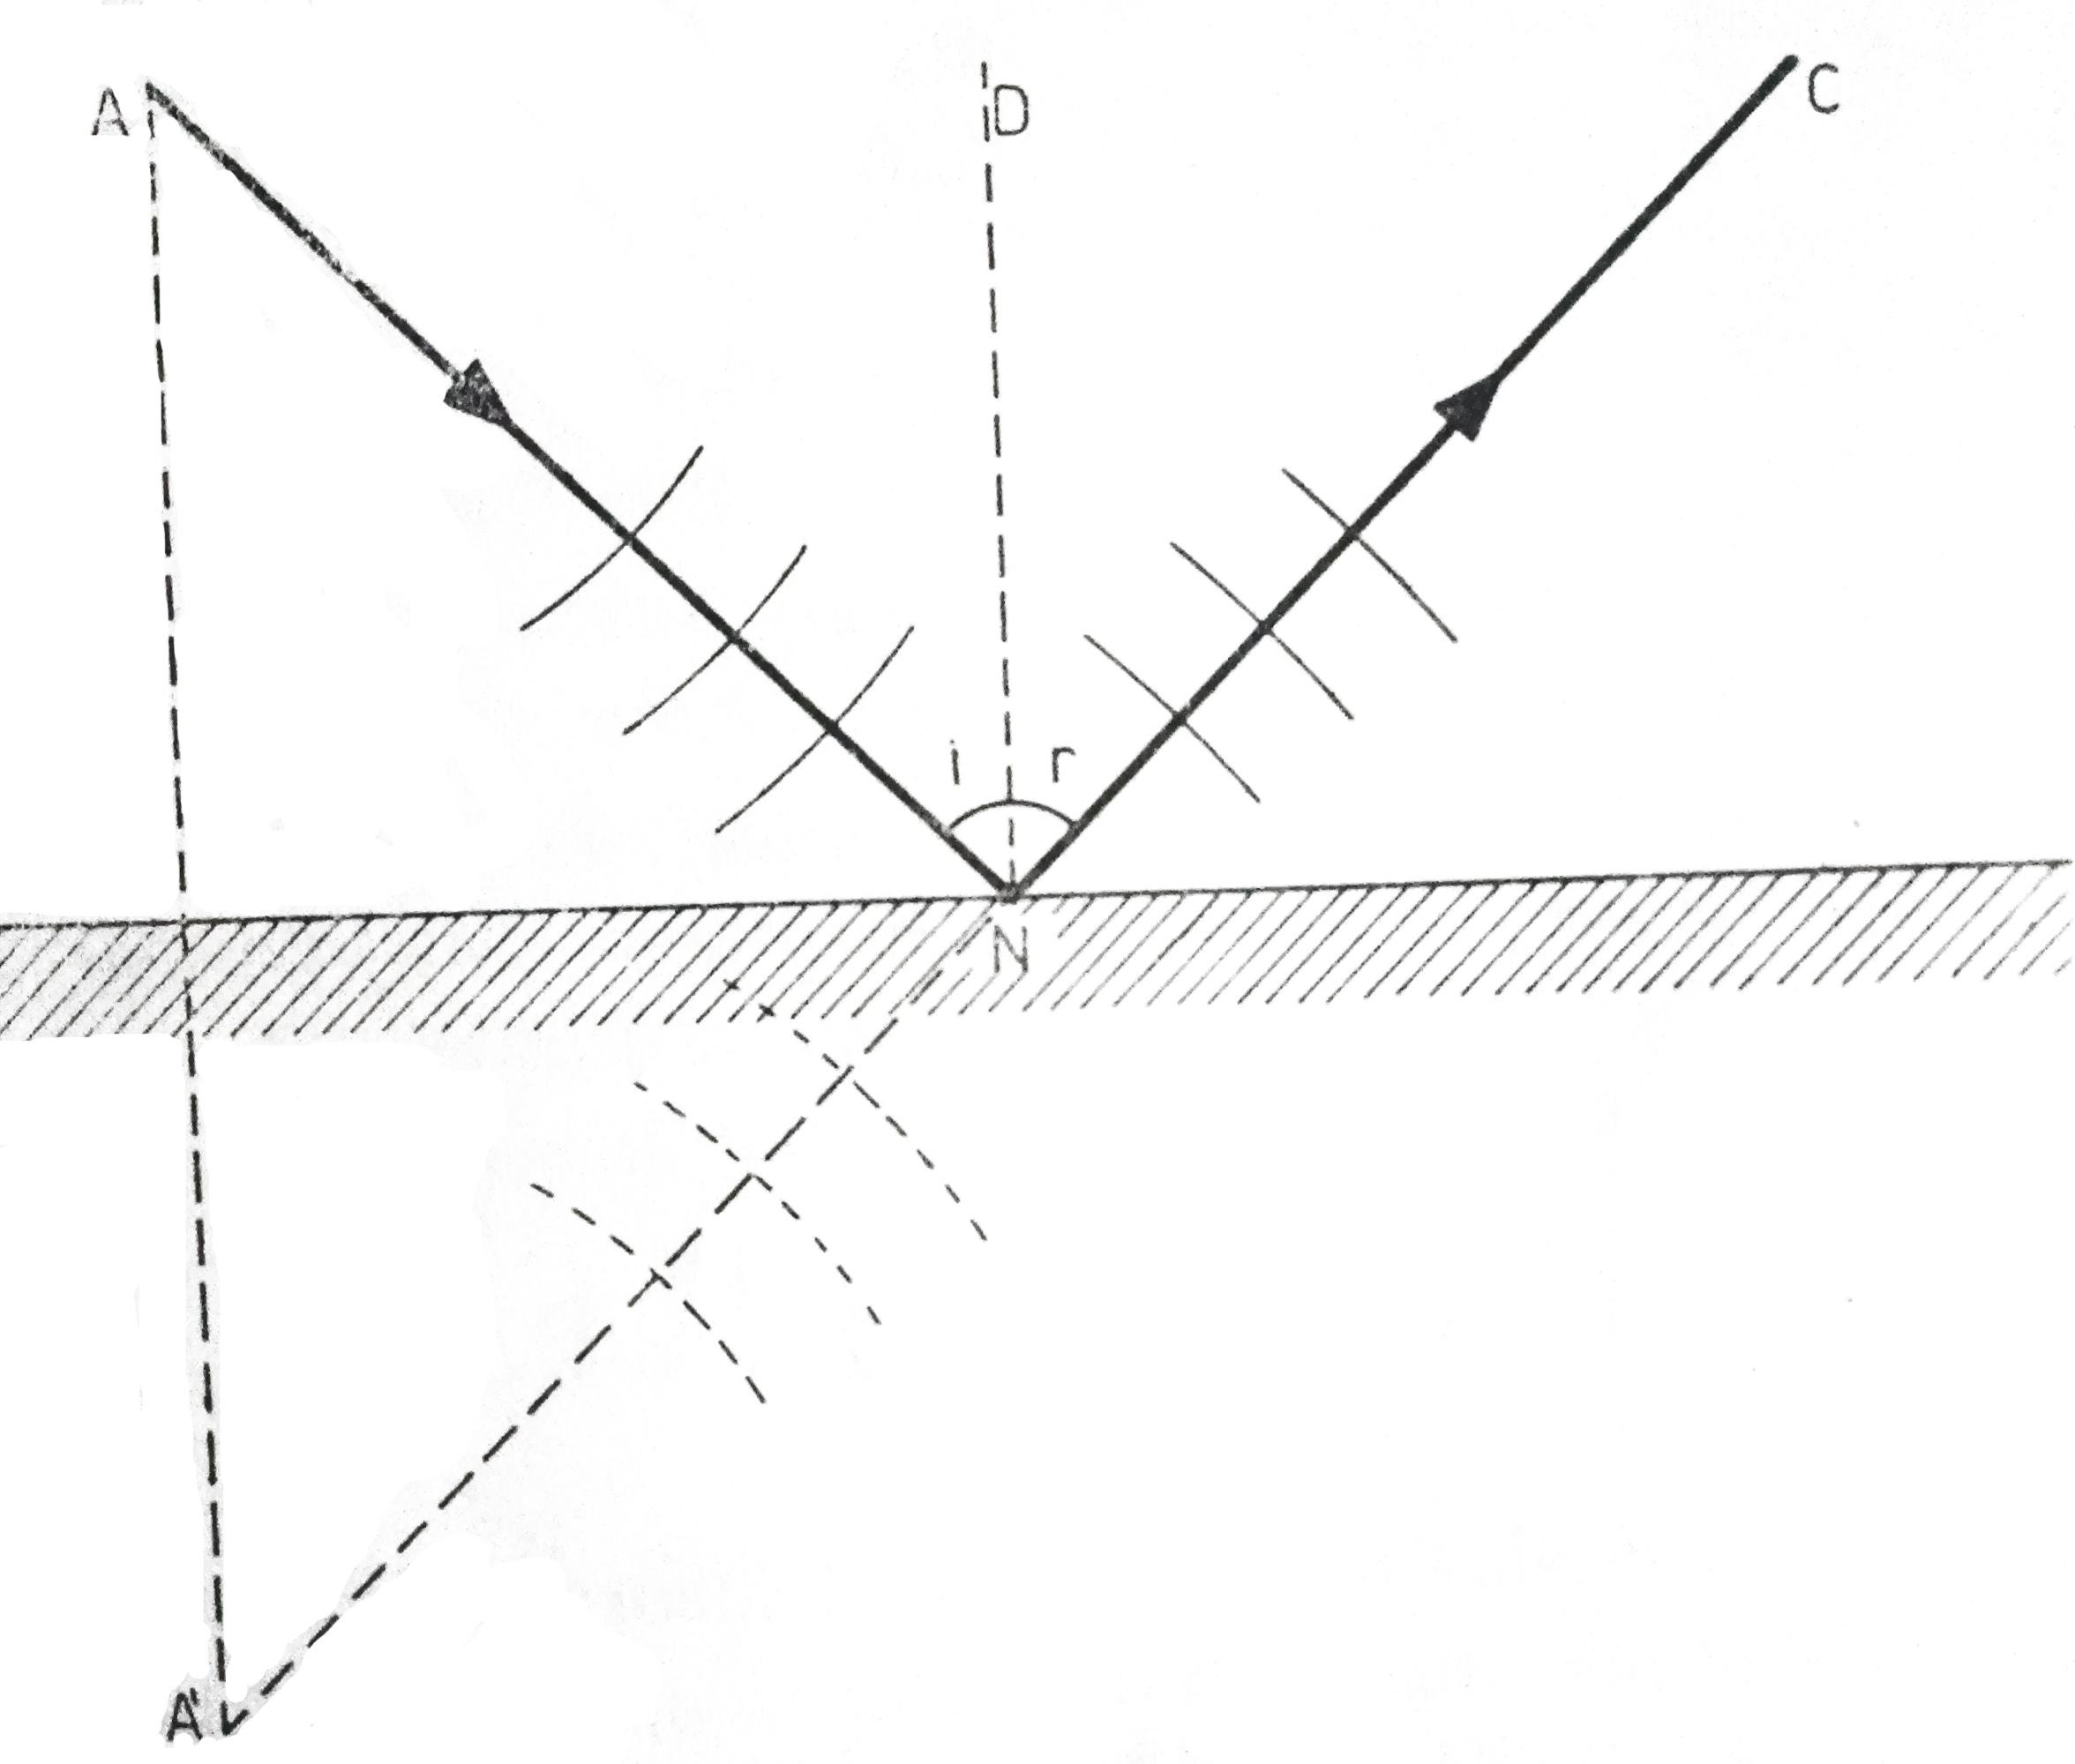
\includegraphics[scale=0.15]{figuras/Reflexao2}
\caption{Reflexão. \cite{silva}}
\label{fig:reflexao2}
\end{figure}

% (Falar sobre o RT60)...

\subsection{Absorção}

Em ambientes fechados, a propagação da onda sonora, a partir da fonte, sofre interferência das ondas que são refletidas nas superfícies que delimitam o recinto como paredes, teto e piso. \cite[pág~231]{bistafa}

Conforme foi ilustrado na figura \ref{fig:reflexao}, quando o som incide sobre uma superfície, uma parte da energia sonora é refletida, enquanto o restante da energia incidente se compõe de duas outras parcelas: a energia sonora absorvida e a energia sonora transmitida para o outro lado da superfície. \cite[pág.~231]{bistafa}

Segundo \cite[pág.~126]{silva}, um material é dito acústico absorvente quando uma grande percentagem da energia sonora que nele incide é retida, degradando-se em energia mecânica ou calorífica, ou ainda transmitindo-se para o outro lado, sendo dele refletida apenas uma pequena parcela.

Chama-se de coeficiente de dissipação sonora, $ \downpropto $, à porcentagem de energia sonora absorvida ou dissipada $ E_{d} $ em um material qualquer, em relação à quantidade de energia acústica  incidente $ E_{i} $ na unidade de área. \cite[pág.~126]{silva}.

\begin{center}
{\Large $ \downpropto = \frac{ E_{d}}{ E_{i}} $}
\end{center}

Coeficiente de reflexão, $ \varrho $, é a relação entre o fluxo de energia acústica refletida, $ E_{r} $, e o fluxo de energia acústica incidente, $ E_{i} $, na unidade de área. \cite[pág.~232]{bistafa}

\begin{center}
{\Large $ \varrho = \frac{E_{r}}{E_{i}} $}
\end{center}

Já o coeficiente de transmissão, $ \tau $, é a relação entre o fluxo de energia acústica transmitida, $ E_{t} $, e o fluxo de energia acústica incidente, $ E_{i} $, também, na unidade de área. \cite[pág.~127]{silva}.
\begin{center}
{\Large $ \tau = \frac{E_{t}}{E_{i}} $}
\end{center}

O coeficiente de absorção acústica, $ \propto $, é a soma dos coeficientes de dissipação, $ E_{d} $, e de transmissão, $ E_{t} $, isto é, a diferença entre a energia acústica incidente e a refletida. \cite[pág.~231]{bistafa}.

\begin{center}
{\Large $ \propto = \downpropto + \tau = \frac{E_{i} - E_{r}}{E_{i}} = 1 - \frac{E_{r}}{E_{i}}~ou~1 - \varrho $}
\end{center}

A soma dos 3 coeficientes descritos acima é:

\begin{center}
{\Large $ \downpropto + \varrho + \tau = \frac{E_{d}}{E_{i}} + \frac{E_{r}}{E_{i}} + \frac{E_{t}}{E_{i}} = 1 $}
\end{center}

Cada material tem um coeficiente de absorção e o seu valor não é constante, pois varia com a frequência do som incidente. Uma superfície, teórica, infinitamente rígida e polida, seria totalmente refletora e seu coeficiente de absorção seria nulo. Já uma janela aberta de um recinto qualquer, teria esse coeficiente igual a 1, o que significa que $ 100\% $ da energia incidente passa para o outro lado, isto é, para o lado de fora. \cite{silva}.

\section{Simulação}

A simulação computacional possui diversos conceitos por diferentes autores, porém, em sua grande maioria, acabam por convergir para o fato de que a simulação contribui para a resolução de problemas complexos \cite{carvalho}. A seguir serão apresentadas as visões de alguns autores a respeito do conceito de simulação.

De acordo com \cite{schriber}, simulação pode ser definida da seguinte maneira: "simulação implica na modelagem de um processo ou sistema, de tal forma que o modelo imite as respostas do sistema real numa sucessão de eventos que ocorrem ao longo do tempo".

Segundo \citeonline{law}, simulação é a imitação de um sistema real, modelado em computador, para avaliação e melhoria de seu desempenho. Ou seja, simulação é a representação de um processo do mundo real para um ambiente controlado onde se pode estudar o comportamento do mesmo, sob diversas condições, sem riscos físicos e/ou grandes custos envolvidos. \cite{torga}.

Segundo \citeonline{torres}, computadores são ótimas ferramentas para simular processos do mundo em que vivemos. De acordo com \citeonline{carvalho}, atualmente, simulação é praticamente sinônimo de simulação computacional digital.

\subsection{Simulação acústica}

A acústica geométrica de salas é um modelo de representação acústica de ambientes fechados onde o conceito de onda sonora é substituído pelo conceito de raio sonoro. \cite{torres}

Dependendo da simplicidade do modelo, a utilização de ferramentas matemáticas como cálculo, álgebra ou probabilidade podem ser suficientes para se obter uma resposta exata a respeito de parâmetros como o tempo de reverberação do som em um ambiente. Essa resposta exata é conhecida como solução analítica do modelo. \cite{torres}

Apesar de ser possível obter resultados utilizando ferramentas matemáticas, é muito raro encontrar sistemas no mundo real que possam ser representados por modelos simples o suficiente para serem resolvidos de forma analítica, pois algumas equações clássicas da acústica de salas não são suficientes para oferecer bons resultados quando as salas assumem geometria complexa. \cite{bastos}

Segundo \citeonline[pág.~5]{torres}, para modelos mais complexos, a simulação é uma ferramenta poderosa que pode ajudar a obter mais informações a respeito de tais processos, como ocorre em simulação acústica, tornando possível prever a acústica de salas complexas.

\begin{citacao}
\begin{normalsize}
"Para que os parâmetros acústicos de um ambiente possam estar de acordo com os padrões previstos para sua finalidade, é recomendável que se faça uma predição do seu comportamento acústico, através de modelos de simulação, para que sejam obtidos resultados com boa precisão em um tempo de processamento relativamente curto, reduzindo custos e aumentando a eficiência dos projetos, quando da seleção correta e quantidade certa de material a ser utilizada para se efetuar tratamentos acústicos nesse ambiente." \cite{bastos}.
\end{normalsize}
\end{citacao}

O avanço na capacidade de processamento dos computadores atuais os tornou capazes de calcular os mais diversos e complexos efeitos da propagação de ondas. Métodos numéricos são capazes de transportar a realidade física para a linguagem computacional. \cite{camilo}.

\section{Sistemas Multiagentes}

Sistemas multiagentes são sistemas compostos de vários elementos de computação interagindo entre si, conhecidos como agentes. Agentes são sistemas computacionais com dois recursos importantes. Primeiramente, eles são pelo menos a certo ponto, capazes de realizar ações autônomas, ou seja, capazes de decidir por si mesmos o que eles precisam fazer a fim de satisfazer seus objetivos de projeto. Em segundo lugar, eles são capazes de interagir com outros agentes, não simplesmente pela troca de dados, mas por se envolver em análogos do tipo de atividade social que todos nós colocamos em nosso dia a dia: a cooperação, coordenação, negociação, dentre outros. \cite{multiagentes}.

Segundo \citeonline{multiagentes2}, "Agentes" são entidades autônomas, computacionais. Dizer que os agentes são entidades computacionais simplesmente significa que existem na forma de programas que são executados em dispositivos de computação. Dizer que eles são autônomos significa que até certo ponto eles têm controle sobre seu comportamento e podem agir sem a intervenção de seres humanos ou outros sistemas. Agentes buscam atingir objetivos ou realizar tarefas, a fim de encontrar seus objetivos de projeto, e em geral, essas metas e tarefas podem ser tanto complementares, como conflitantes.

Dizer que os agentes são inteligentes não significa que eles são omnisciente ou onipotente, nem significa que eles nunca falham. Pelo contrário, significa que eles operam de forma flexível e racional em uma variedade de circunstâncias ambientais, dada a informação que eles têm e as suas capacidades perceptivas e eficazes. O foco principal está em processos como a resolução de problemas, planejamento, pesquisa, tomada de decisões e de aprendizagem que tornam possível para os agentes, mostrar flexibilidade e racionalidade em seu comportamento, e sobre a realização de tal processo em cenários multiagentes. \cite{multiagentes2}.

Agentes também interagem entre si, isto é, os agentes podem ser afetados por outros agentes em busca de atingir seus objetivos e executar suas tarefas. A interação pode ocorrer indiretamente, através do meio ambiente em que estão embutidas, ou diretamente, através de uma linguagem comum. \cite{multiagentes2}.

Um sistema multiagentes pode ser descrito como uma comunidade de agentes autônomos, onde estes interagem, se organizam e se comunicam, competindo ou cooperando uns com os outros, a fim de alcançar o objetivo proposto para esse sistema. \cite{thomaz}.

A área de sistemas multiagentes é um promissor domínio tecnológico para uso em performances musicais interativas. Essa tecnologia vem sendo utilizada para resolver problemas musicais de escopo específico e alcance limitado, como por exemplo, a simulação de instrumentos e o acompanhamento musical automático. \cite{thomaz}.

\section{Considerações finais}

Prever o comportamento do som dentro de um ambiente fechado vem se tornando uma necessidade cada vez mais notável, porém, não é trivial. Para isto, está sendo cada vez mais comum o uso de simuladores que auxiliem os profissionais da área da acústica arquitetônica na análise do comportamento sonoro em seus projetos.

O paradigma de programação multiagentes apresenta um grande potencial para tal finalidade, apesar de ter sido pouco explorado na área de simulação de ambientes acústicos. As capacidades de autonomia, paralelismo e cooperação dos agentes, também podem ser percebidas no comportamento sonoro em um ambiente, o que demonstra uma promissora capacidade de representação do som dentro de ambientes fechados..